\section{Conclusiones}

\quad Esta aplicación a resultado apasionate, pues realmente creo que me ha hecho crecer como desarrollador. Digo esto, porque trabajar en un proyecto tuyo, que sabes que quieres hacer y que tu mismo propusiste, puede ser abrumador, pero acaba sacando lo mejor de ti.\\

\quad Por la falta de potencia de procesamiento, tanto del equipo de desarrollo como del movil con el que se iba a trabajar, ubo una idea uqe se tuvo que desechar, que era aplicar Raytracing al concepto de 8D. Esto se va a desarrollar ahora mismo en el apartado siguiente.\\

\subsection{Lineas futuras, Ray tracing}

\subsubsection{Definición y planteamiento para sonido}

\quad El raytracing es un algoritmo para síntesis de imágenes tridimensionales propuesto inicialmente por Turner Whitted en 1980. Está basado en el algoritmo de determinación de superficies visibles de Arthur Appel denominado Ray Casting (1968), en el que se se determinan las superficies visibles en la escena que se quiere sintetizar trazando rayos desde el observador (cámara) hasta la escena a través del plano de la imagen. Se calculan las intersecciones del rayo con los diferentes objetos de la escena y aquella intersección que esté más cerca del observador determina cuál es el objeto visible.\\

\quad En el Raytracing se extiende la idea de trazar los rayos para determinar las superficies visibles con un proceso de sombreado (cálculo de la intensidad del píxel) que tiene en cuenta efectos globales de iluminación como pueden ser reflexiones, refracciones o sombras arrojadas. Para simular los efectos de reflexión y refracción se trazan rayos recursivamente desde el punto de intersección que se está sombreando dependiendo de las características del material del objeto intersecado. Para simular las sombras arrojadas se lanzan rayos desde el punto de intersección hasta las fuentes de luz. Estos rayos se conocen con el nombre de rayos de sombra (shadow rays).\\

\quad Se puede apreciar que en los parrafos anteriores solo se habla de gráficos, lo cuál plantea cómo aplicar esto a sonido. En realidad el concepto es muy similar al lo anterior, se imiten los rayos, pero determinamos las variaciones del sonido por los rebotes en los diferentes elementos en una habitación, determinando el ángulo de entrada más optimo para ese fin.\\

\begin{figure}[htb]
	\centering
	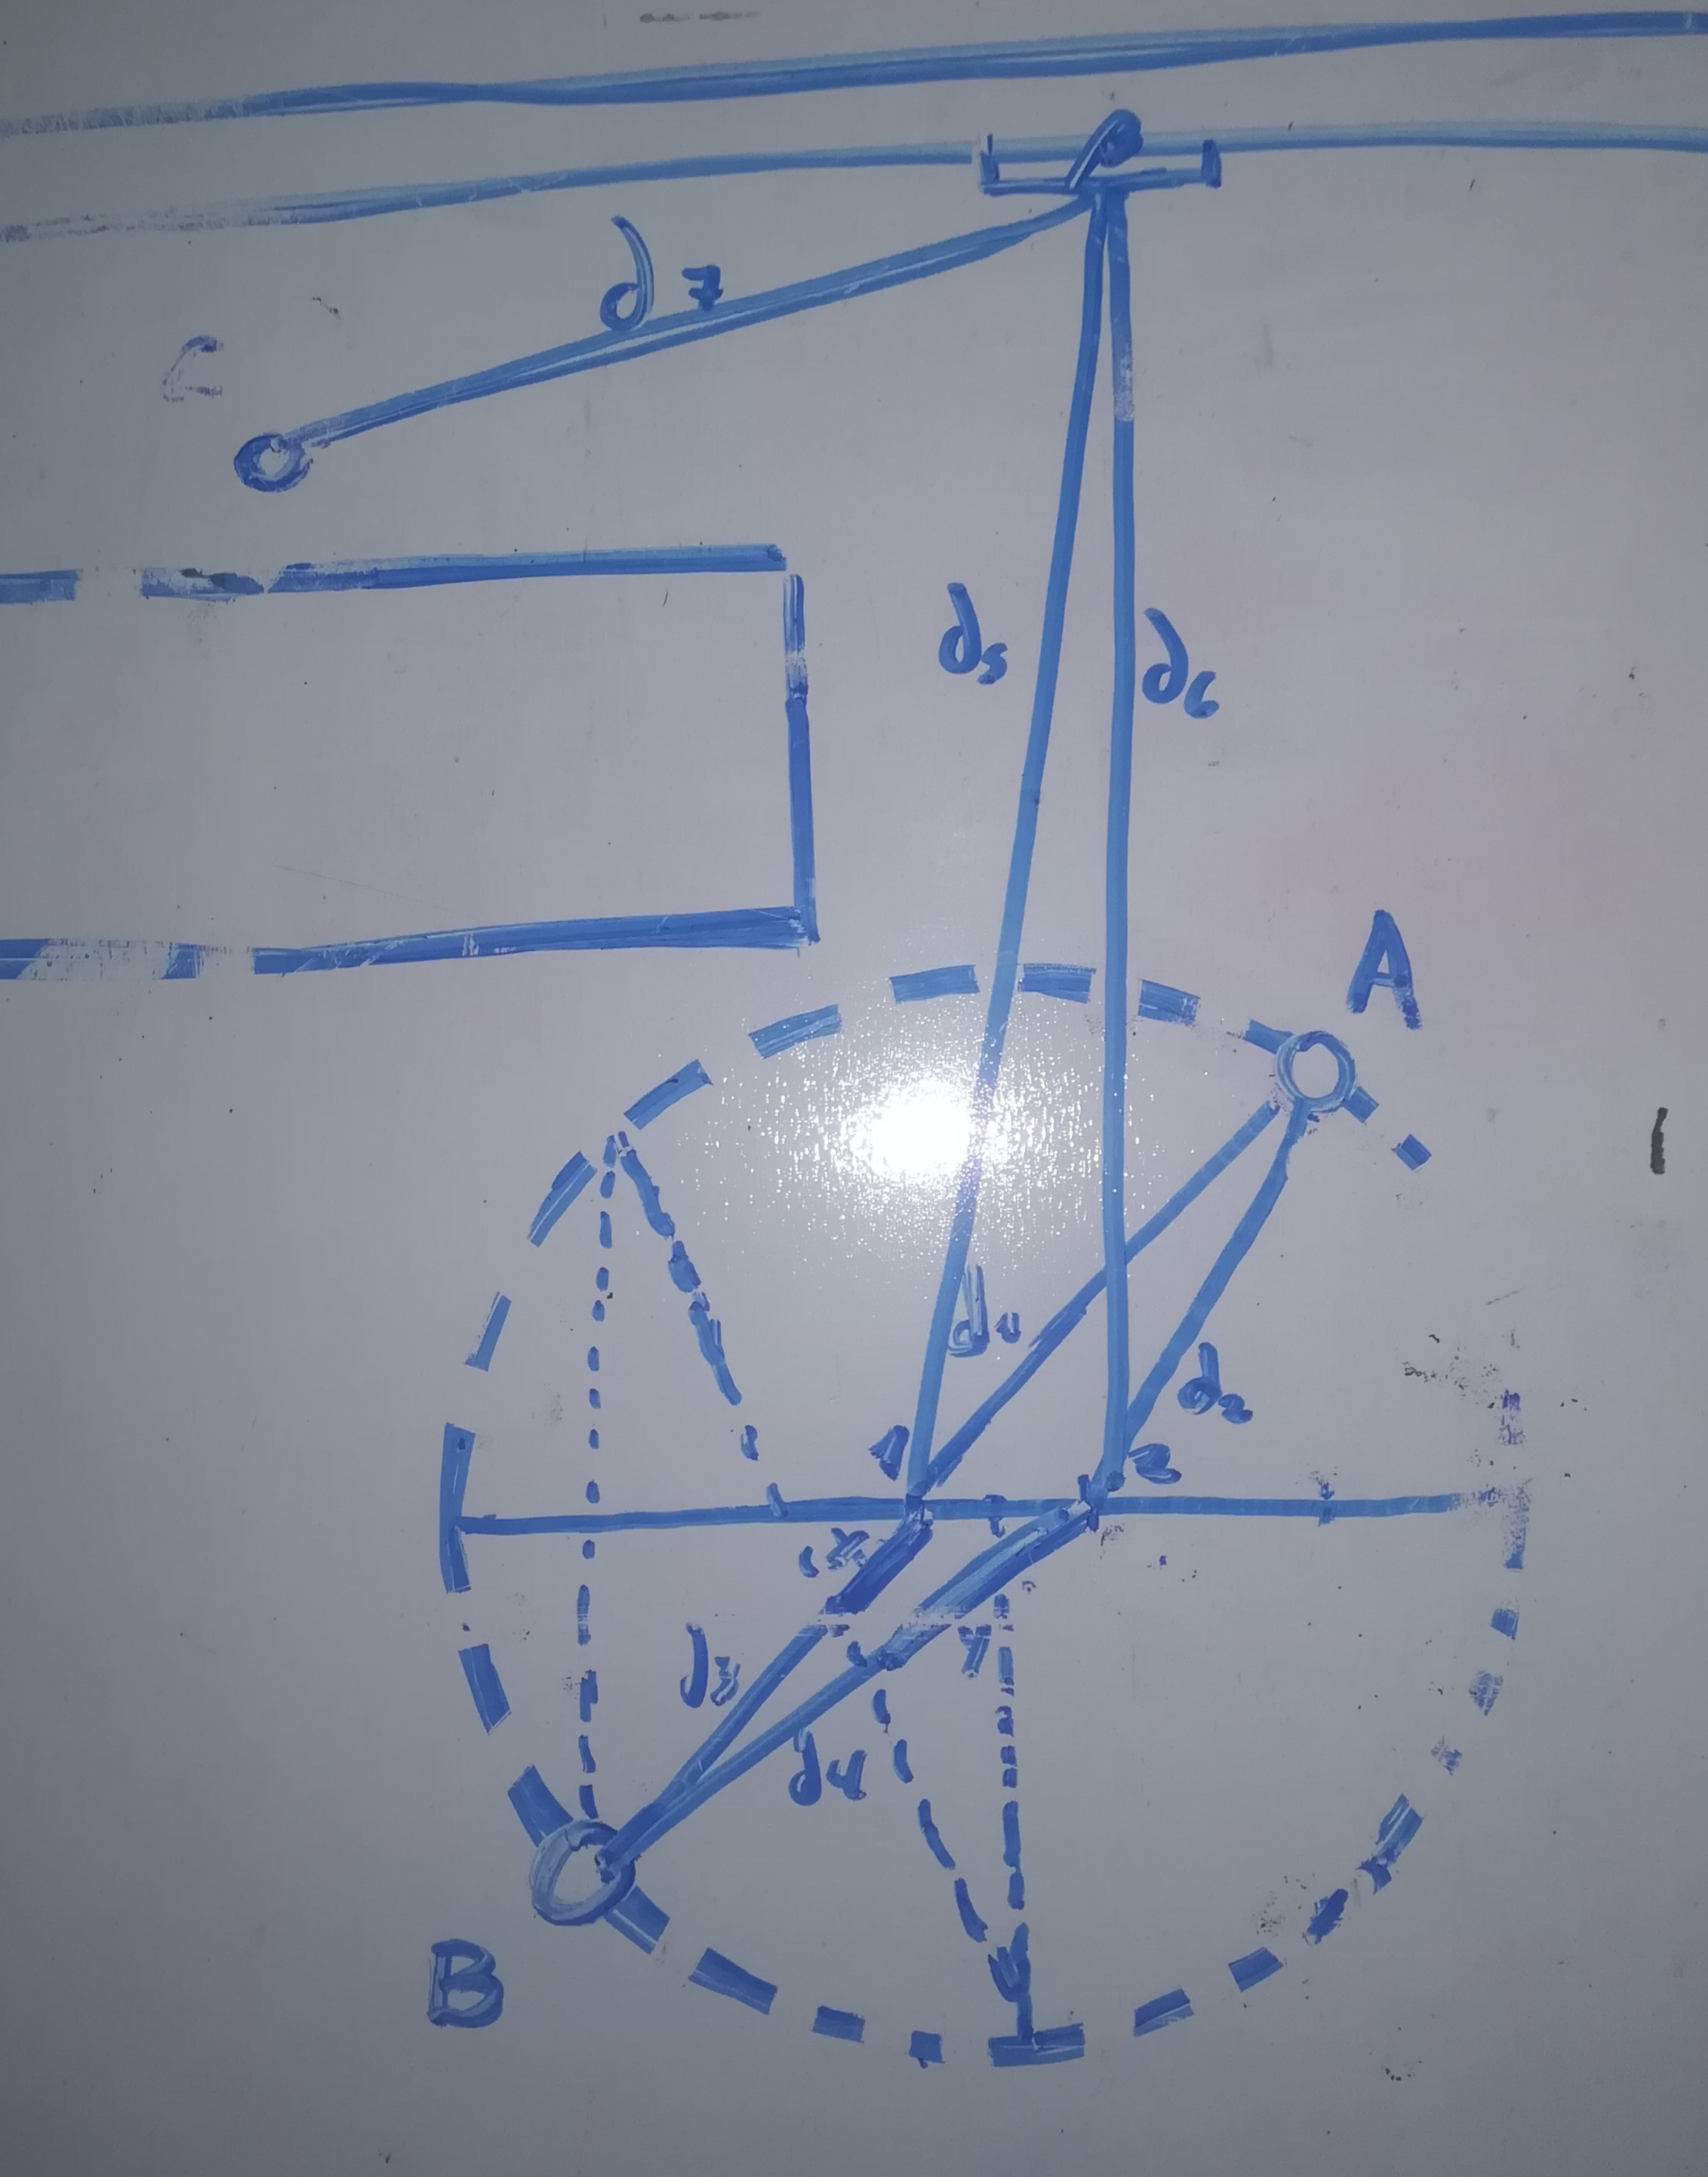
\includegraphics[width=0.5\textwidth]{./imagenes/pizarra}
	\caption{Esquema conceptual en pizarra del raytracing}
\end{figure} 

\quad Gracias a la industria del videojuego, no estamos lejos de poder disfrutar del raytracing de una forma más común, ya que juegos como Cyberpunk 2077 (a día de la redacción de este documento, el juego no ha salido al mercado) plantean el uso de esta tecnología, pero los equipos de los que disponen los jugadores aún no estan a la altura de una carga computacional tan grande. Con todo, solo se puede decir que el cielo es el límite, y que en un futuro no tan lejano, todo lo plateado sobre esta tenología que suena a ciencia ficción, disfrutaremos de todo esto como si fuera lo más común y normal.\\ 

\newpage


